\documentclass[10pt]{article}
\usepackage{eecs149}
\usepackage{multicol,caption}
\newenvironment{Figure}
  {\par\medskip\noindent\minipage{\linewidth}}
  {\endminipage\par\medskip}
\tikzset{
  >=stealth'
}
\begin{document}
\begin{center}
  \Large Gesture Controlled Driving
\end{center}
\begin{center}
  Ollie Peng, Manish Raghavan, Victor Sutardja
\end{center}
\begin{multicols}{2}
  \section*{Overview}
  Using the Kobuki platform from lab, we built a system by which the Kobuki
  drives in a path drawn by the user. Specifically, the user draws a path in the
  air using a brightly colored object. The Kobuki takes a series of images of
  this path using a webcam mounted on its frame. These images are streamed to a
  laptop which performs the image-processing needed to detect the object used
  for drawing. The points from the images are interpolated into a smooth path.
  Using feedback from the OptiTrack camera system, the Kobuki is instructed to
  drive along this path, correcting for any errors in real time.

  \section*{Setup}
  \begin{Figure}
    \begin{tikzpicture}[->,shorten >=1pt,auto,node distance=2cm, thin]
      \node (m) [rectangle,draw] at (0,0) {Mac};
      \node (k) [rectangle,draw] at (2,0) {Kobuki};
      \node (w) [rectangle,draw] at (-3.5,0) {Windows};
      \node (o) [rectangle,draw] at (-3.5,2) {OptiTrack};

      \path
      (k) edge [bend right=30] node [above] {orientation} (m)
      (m) edge [bend right=30] node [below] {radius and speed} (k)
      (w) edge node [below,align=center] {position and\\orientation} (m)
      (o) edge node [right,align=center] {full tracking\\data} (w)
      ;
    \end{tikzpicture}
    \captionof{figure}{Flow of information} \label{fig:info}
  \end{Figure}

  Figure~\ref{fig:info} shows the flow of information between various devices.
  There are two key design decisions we made in order to overcome challenges we
  faced. First, we streamed the OptiTrack data to a separate Windows machine
  instead of the Mac that was communicating with the data because the frame rate
  from the traking system was too high and would be constantly modifying shared
  variables. Since we were only sending updated commands to the Kobuki once
  every second, we did not need such frequent information, and therefore used
  the Windows machine to sample the data at a lower rate before passing it on
  the Mac. Second, we chose to take orientation data from both the OptiTrack and
  Kobuki. We did so because the orientation from OptiTrack was given in terms of
  quaternions in a rotated axis space, meaning that the standard equations for
  converting to yaw, pitch, and roll no longer applied. Instead, we needed to
  know which quadrant the yaw was in to correct them. As a result, we used the
  orientation from the Kobuki to determine which quadrant it was facing,
  allowing us to use the correct equations to get the true orientation.

  \section*{Image Processing}

  \section*{Spline Interpolation}

  \section*{Timing}

  \section*{Threading}

  \section*{Modeling movement}
  \begin{Figure}
    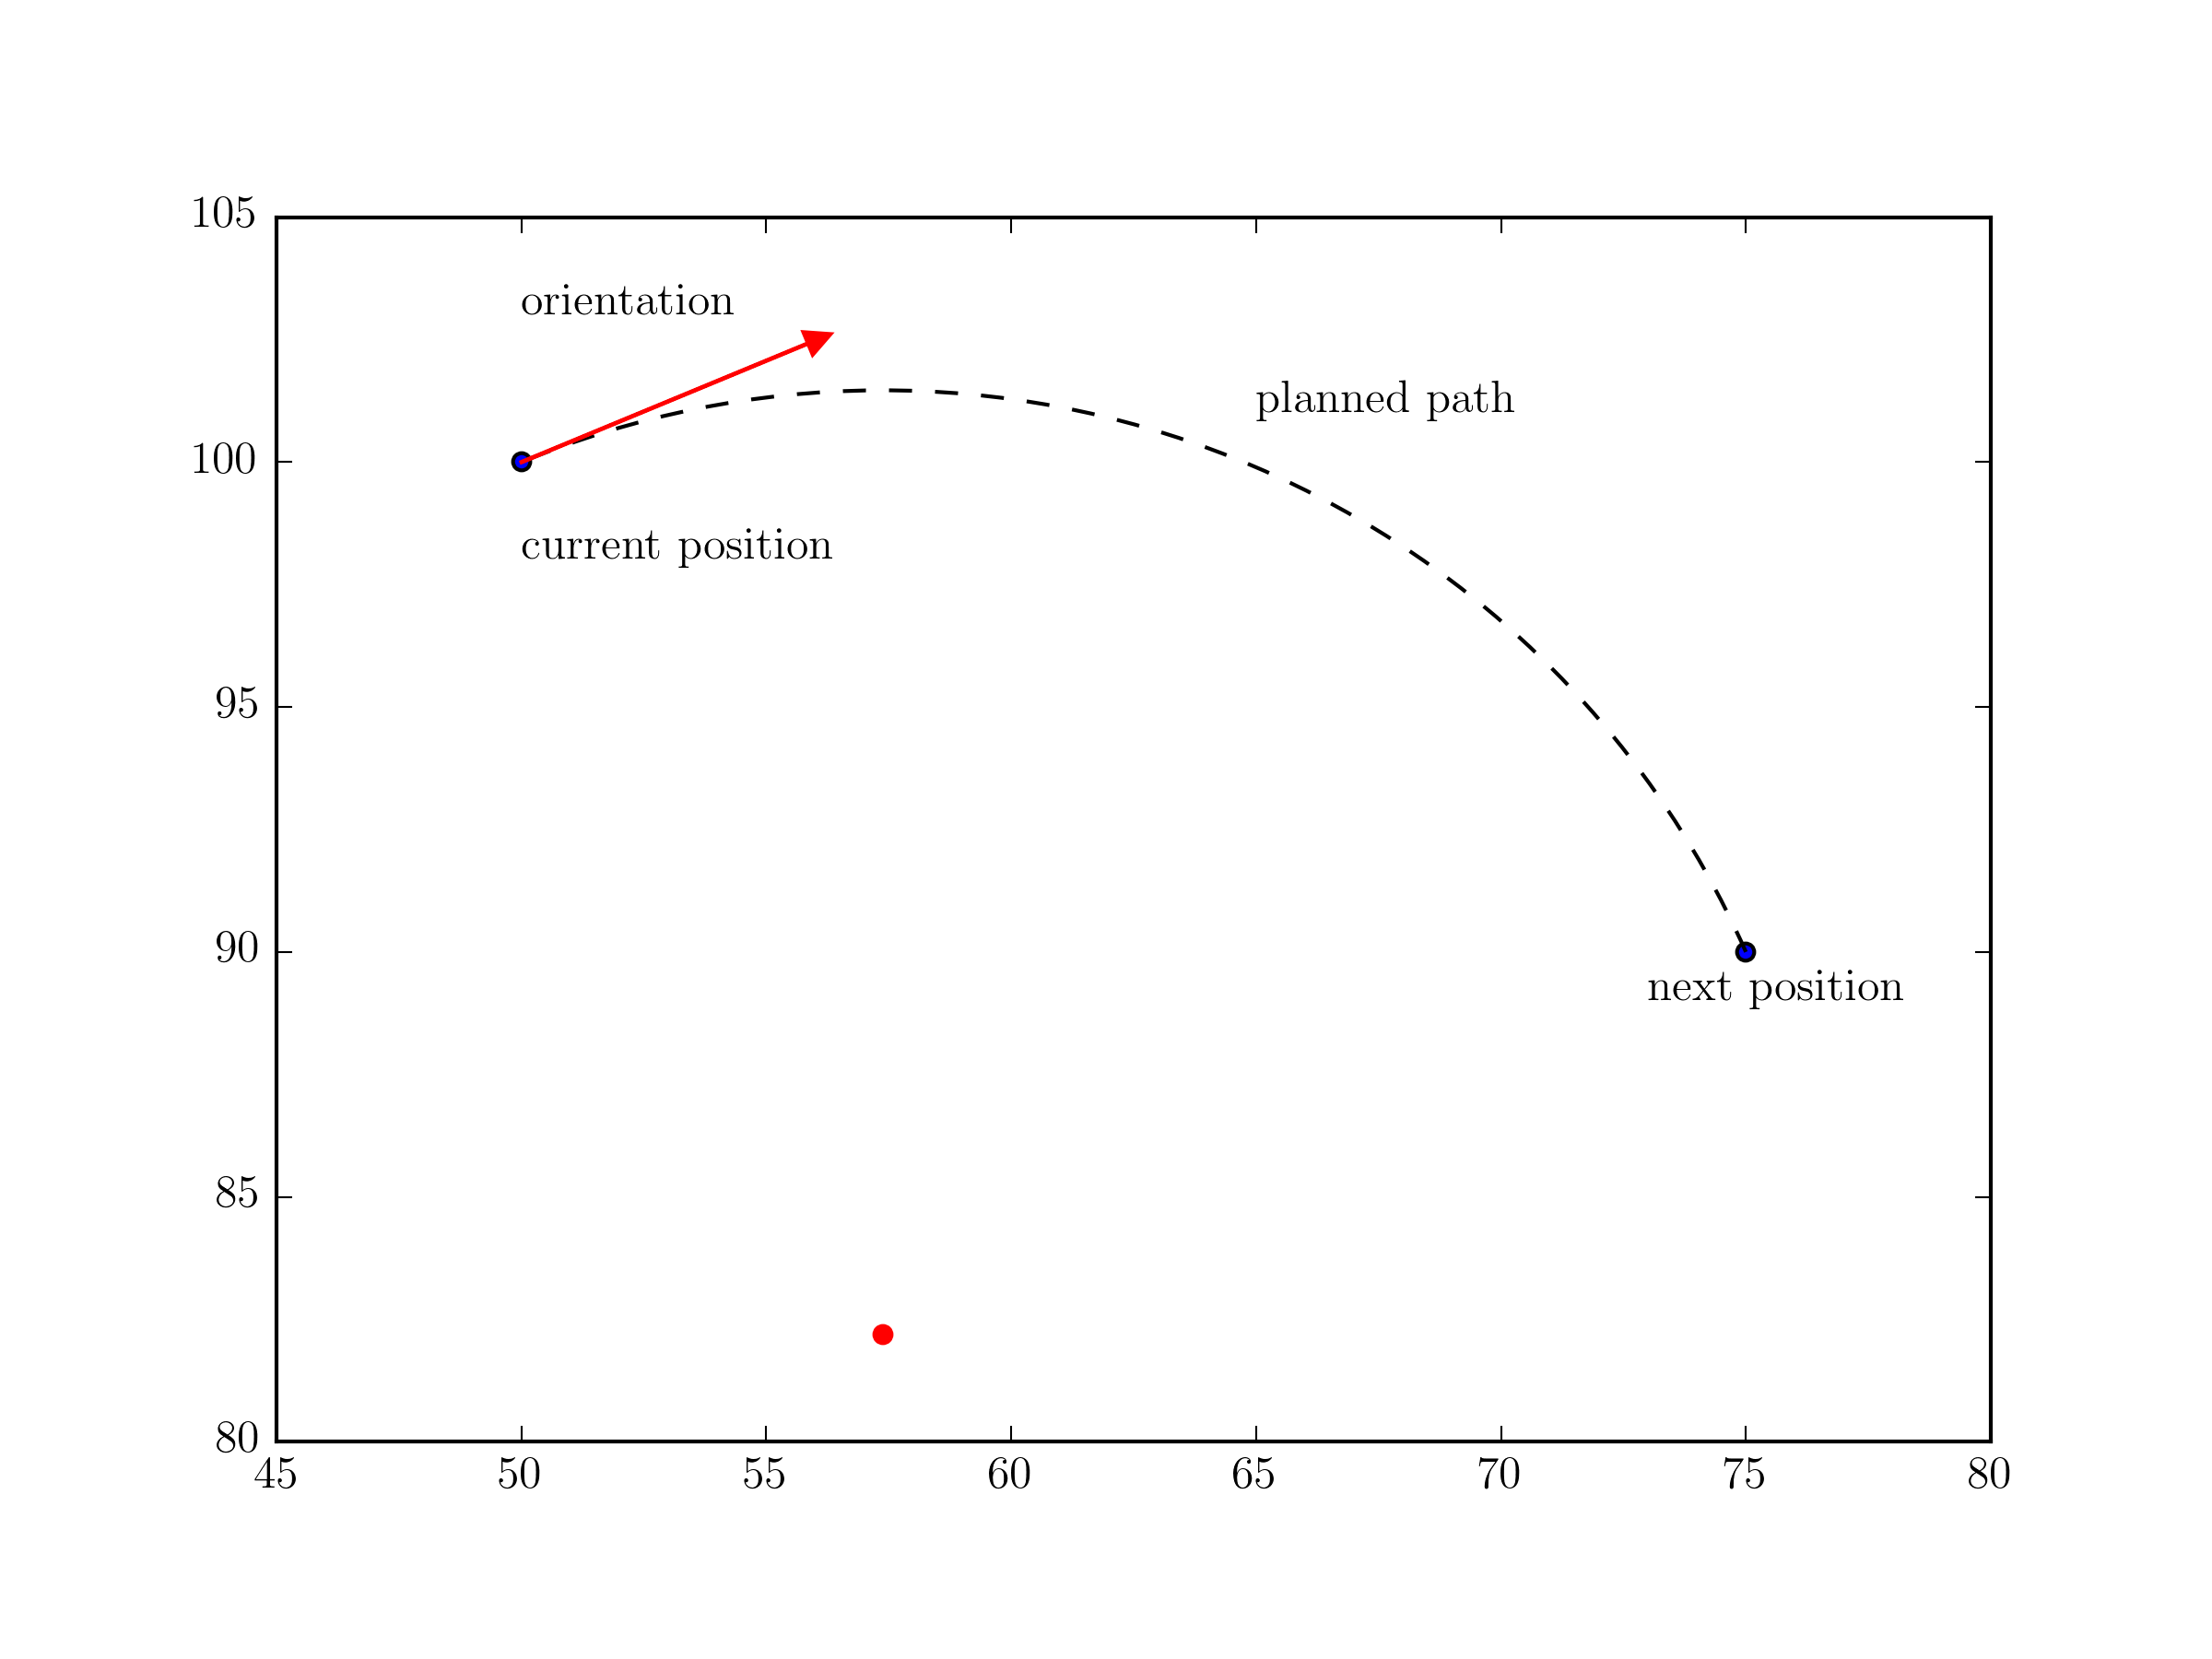
\includegraphics[width=10cm]{../plots/roc.png}
    \captionof{figure}{Movement planning} \label{fig:roc}
  \end{Figure}

  \section*{Results}
\end{multicols}
\end{document}
